\documentclass[aspectratio=169]{beamer}

\usetheme{Madrid}
\usecolortheme{default}
\setbeamertemplate{navigation symbols}{}

\usepackage[utf8]{inputenc}
\usepackage[T1]{fontenc}
\usepackage{graphicx}

\title{CMPE362 HW4\\Audio Speech/Music Separation and Hidden Message Analysis}
\author{Ali Ayhan Günder \\ Student ID: 2021400219}
\institute{CMPE362}
\date{March 16, 2026}

\begin{document}

\begin{frame}
  \titlepage
\end{frame}

\begin{frame}{Spectrograms: Original and Speech-Filtered}
\begin{columns}[T]
  \column{0.5\textwidth}
  \centering
  \textbf{cafe\_sample.wav}\\[2mm]
  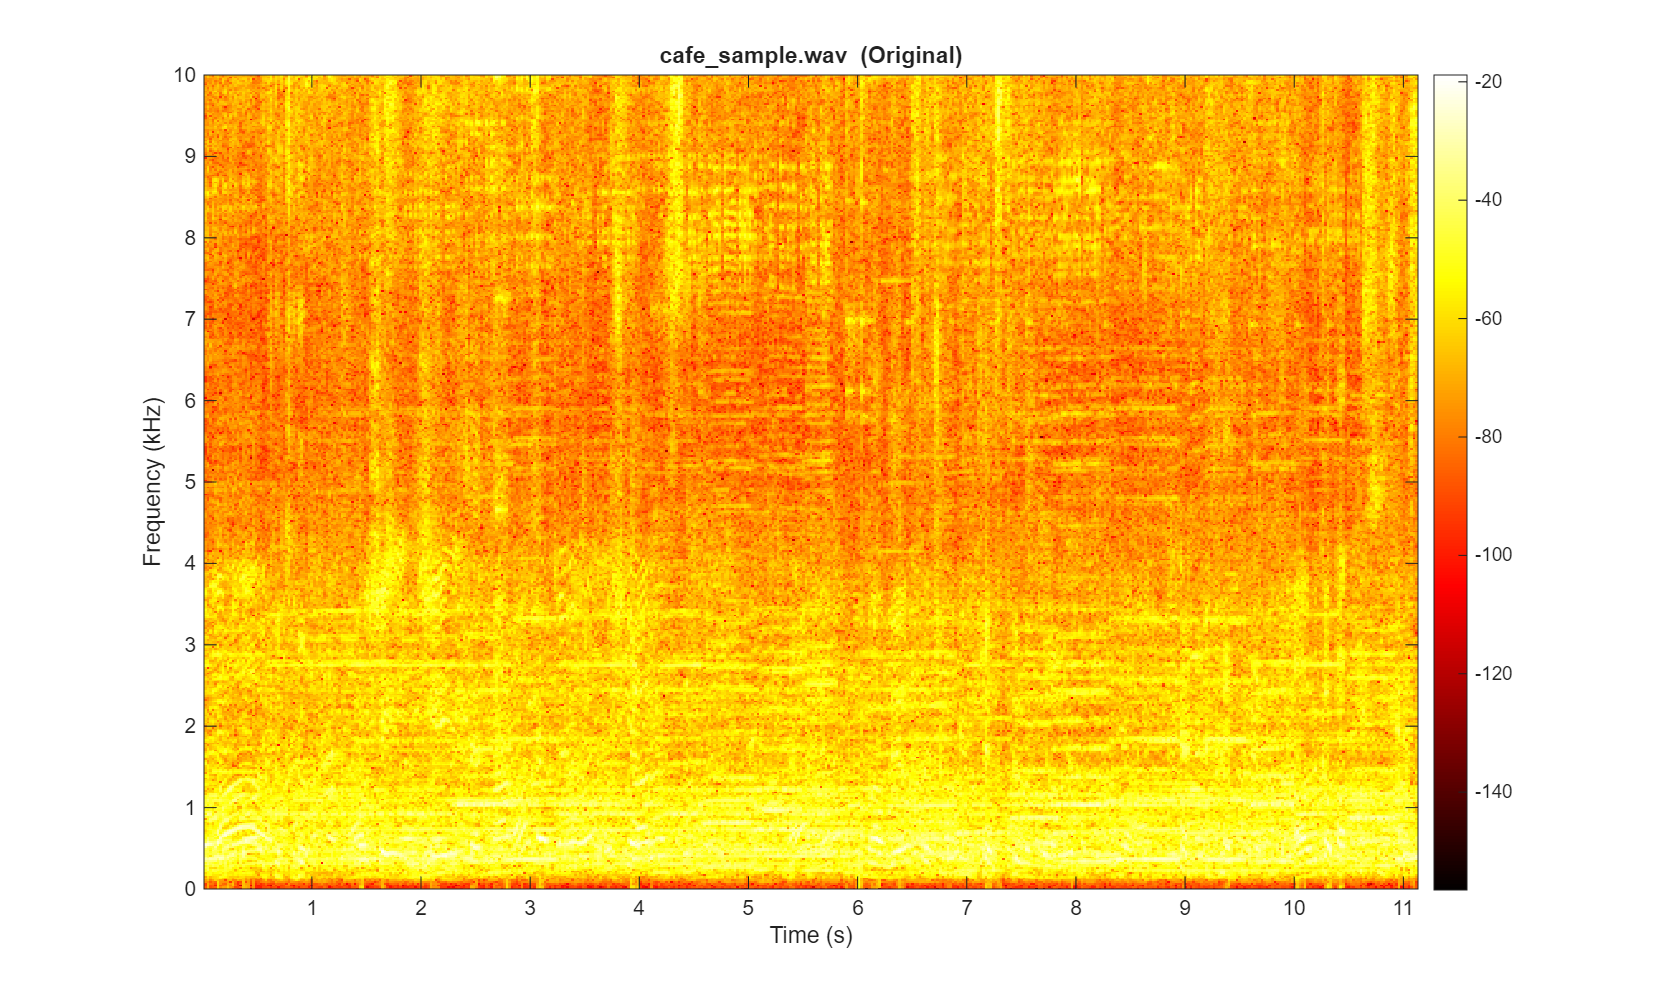
\includegraphics[width=\linewidth,height=0.62\textheight,keepaspectratio]{spectrogram_original.png}

  \column{0.5\textwidth}
  \centering
  \textbf{speech\_filtered.wav}\\[2mm]
  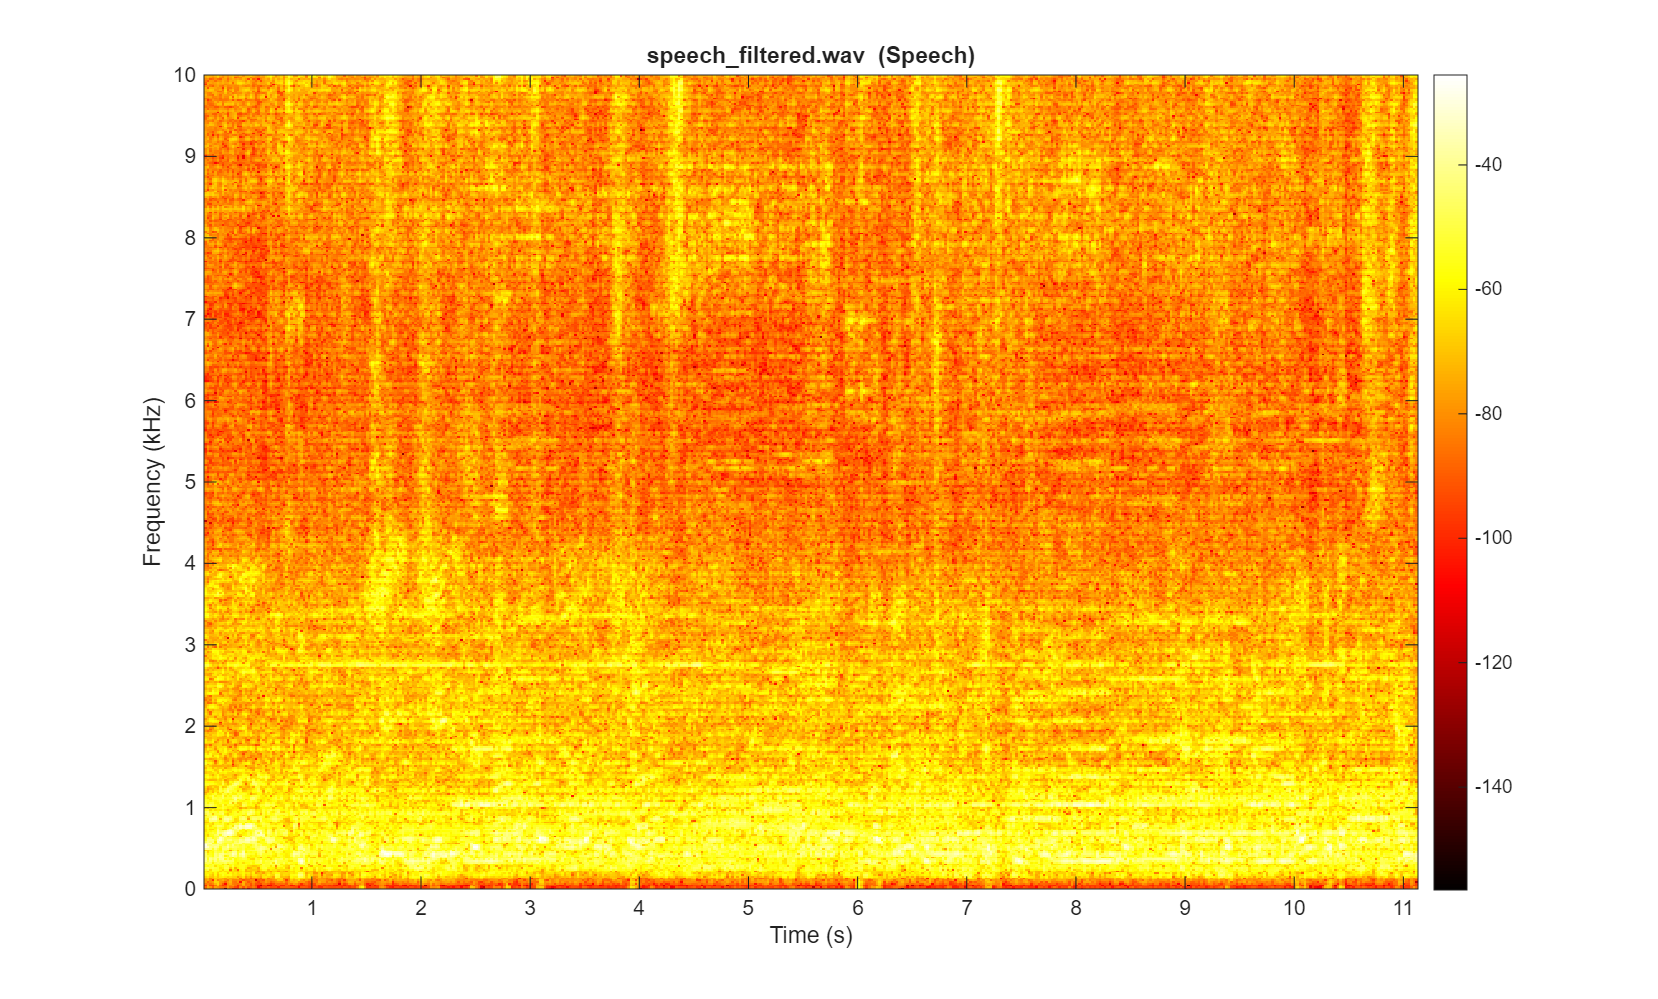
\includegraphics[width=\linewidth,height=0.62\textheight,keepaspectratio]{spectrogram_speech_filtered.png}
\end{columns}

\vspace{1mm}
\footnotesize
\begin{itemize}
  \item Original signal has overlapping speech and music energy.
  \item In speech\_filtered output, background music is attenuated and speech-dominant regions become more prominent.
\end{itemize}
\end{frame}

\begin{frame}{Spectrogram: Music-Filtered (Music-Preserved)}
\begin{columns}[T]
  \column{0.58\textwidth}
  \centering
  \textbf{music\_filtered.wav}\\[2mm]
  
\includegraphics[width=\linewidth,height=0.66\textheight,keepaspectratio]{spectrogram_music_filtered.png}

  \column{0.42\textwidth}
  \small
  \textbf{Observation}
  \begin{itemize}
    \item Harmonic/instrumental structure is preserved more strongly than the original mix.
    \item Speech-like transients/formants are reduced but not fully eliminated.
    \item Some residual overlap remains (expected for single-channel blind separation).
  \end{itemize}
\end{columns}
\end{frame}

\begin{frame}{Method Journey: How I Chose the Best Result}
\footnotesize
\textbf{Goal:} not perfect separation, but the best practical speech/music split from a single mixed recording.

\vspace{1mm}
\textbf{Methods I tested during development}
{\setlength{\itemsep}{0.25em}
\begin{itemize}
  \item Baseline classical filtering: bandpass/bandstop designs (fast, but limited separation when spectra overlap).
  \item STFT mask methods (IRM/ratio masks): improved selectivity in time-frequency domain.
  \item Enhanced variants (e.g., precise/balanced scripts): tuned suppression vs speech quality tradeoff.
  \item Alternative decomposition families: HPSS, NMF, ICA, k-means, and DRNN-based experiments.
\end{itemize}}

\textbf{What I observed}
{\setlength{\itemsep}{0.25em}
\begin{itemize}
  \item Single-method outputs were either under-suppressed (music leakage) or over-processed (robotic artifacts).
  \item Speech and music overlap in the same frequency bands, so frequency-only filters were insufficient.
\end{itemize}}

\textbf{Decision}
{\setlength{\itemsep}{0.25em}
\begin{itemize}
  \item Final speech output: aggressive reference-music cancellation (xcorr lag alignment + scaled subtraction) followed by STFT over-subtraction and gating.
  \item Final music output: reference-stem guided STFT ratio masking (generalized Wiener mask) to retain background music while suppressing foreground speech.
\end{itemize}}
\end{frame}

\begin{frame}[t]{Filters, Frequency Targets, Reasoning, and Process}
\footnotesize
\textbf{Selected best scripts:} \texttt{best/speech\_filter.m} (speech) and \texttt{best/music\_filter.m} (music)

\vspace{1mm}
\begin{columns}[T]
  \column{0.49\textwidth}
  \textbf{Methods/filters used}
  {\setlength{\itemsep}{0.2em}
  \begin{itemize}
    \item Speech: xcorr lag alignment + least-squares gain scaling + phase-inversion subtraction
    \item Speech: STFT over-subtraction + hard gating + high-frequency cutoff
    \item Music: STFT ratio mask / generalized Wiener mask (p=2.5) using website stems as references
    \item Reconstruction: overlap-add iSTFT, normalization
  \end{itemize}}

  \textbf{Frequency targets}
  {\setlength{\itemsep}{0.2em}
  \begin{itemize}
    \item Speech (v12): aggressive suppression of music residue; hard mute above 3.2 kHz to reduce piercing instrumentation
    \item Music (v5): preserve harmonic/instrumental content via ratio masks; suppress speech residue using oracle stems
  \end{itemize}}

  \column{0.49\textwidth}
  \textbf{Reasoning and process}
  {\setlength{\itemsep}{0.3em}
  \begin{itemize}
    \item Music is more repetitive/harmonic; speech is more transient.
    \item Frequency-only filtering was not sufficient due to overlap.
    \item Combining complementary masks improved suppression/intelligibility balance.
    \item Soft masks reduced harsh artifacts compared to binary masking.
    \item Final pipeline was selected as the best overall tradeoff.
  \end{itemize}}
\end{columns}
\end{frame}

\begin{frame}{Bonus: Hidden Message Decoding}
\textbf{Decoded message (best interpretation):} \Large \textbf{I SEE YOU}

\vspace{2mm}
\normalsize
\textbf{Process summary}
\begin{itemize}
  \item Focused ultrasonic BFSK-style demodulation around 17.6 kHz.
  \item Stability sweeps: carrier (17580--17620 Hz), symbol time (0.155--0.190 s), windows (40/50/60/80 ms).
  \item Cross-checked with DTMF/Morse/LSB scans; none produced a clearer full phrase.
  \item Turkish-language interpretation from noisy pattern \texttt{L?ISME?O}: probable key/message is \textbf{G\"UL\"UMSE} (\"Smile\").
\end{itemize}

\textbf{Confidence}
\begin{itemize}
  \item Medium-high: core pattern is repeatable, but decoding is sensitive to timing/demodulation parameters.
\end{itemize}
\end{frame}

\end{document}